\documentclass[../main/thesis.tex]{subfiles}
\begin{document}

\chapter{3DMiMic Layouts}
\label{a-3dmimic-layout}

\begin{figure}[h]
	\centering
	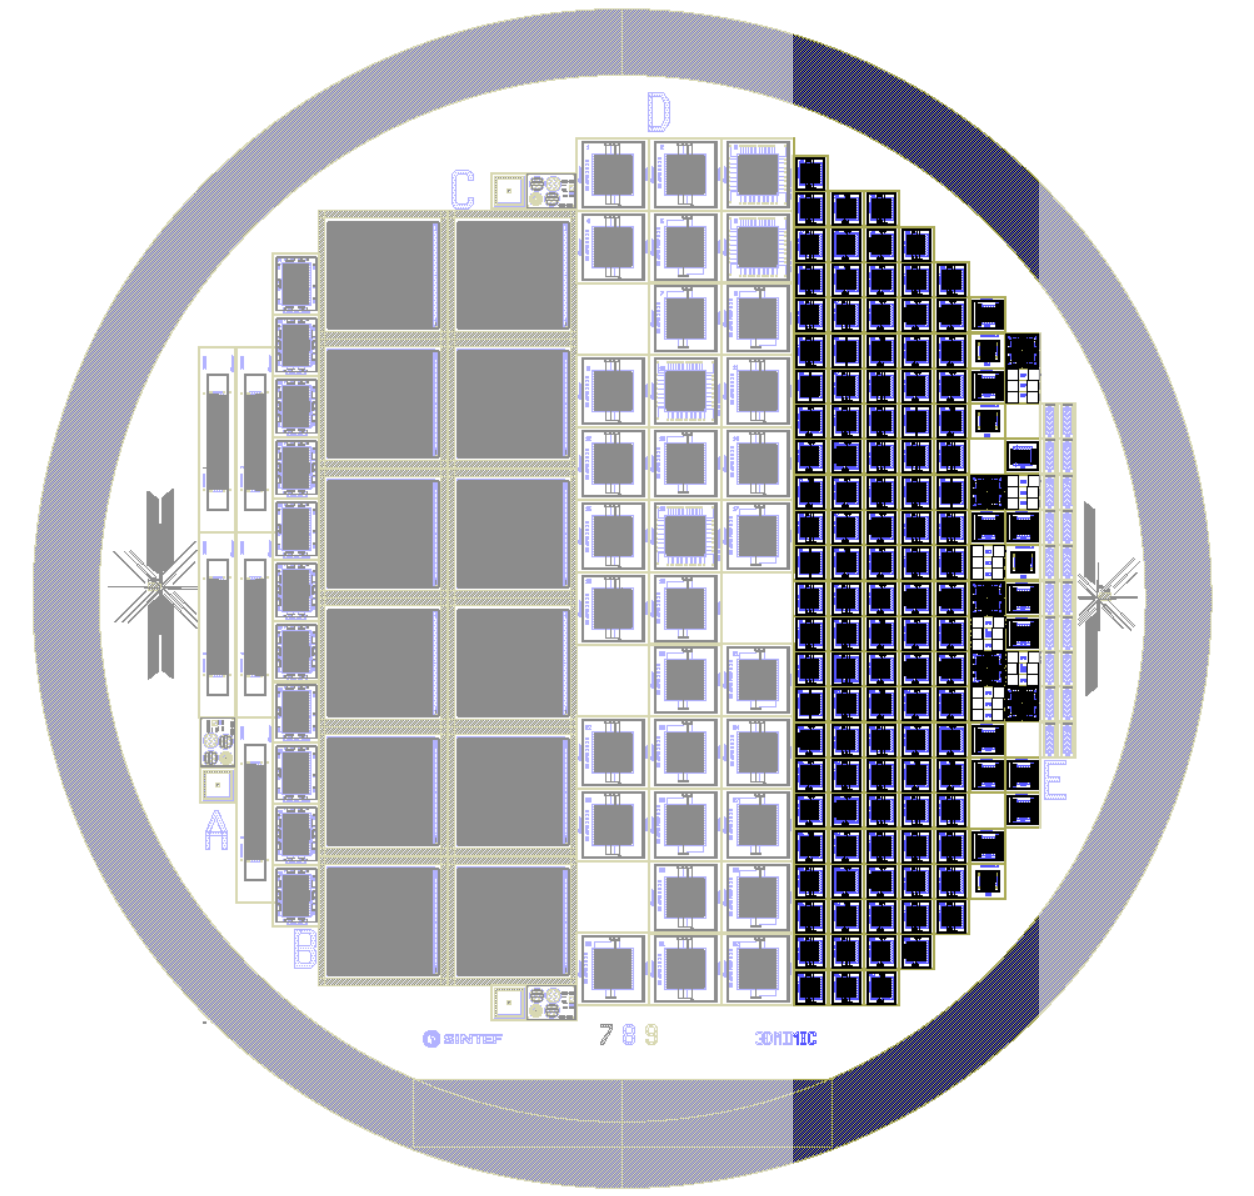
\includegraphics[width=1\textwidth]{layout/wafer_2.png}
	\caption{3DMiMic wafer.}
	\label{fig-wafer} 
\end{figure}

Figure \ref{fig-wafer} shows a whole 3DMiMic wafer. The highlighted area are the detectors that are relevant for this thesis. The large detectors on the left are made to be bump bonded with a Medipix chip. Figures \ref{fig-mic-array-1} to \ref{fig-mic-3D} show some of the different layouts in the highlighted area. The detectors with "$\_$L" in the name are of the "30 $\mu$m" size, while the others are of the "15 $\mu$m" size, see figure \ref{fig-top-both}. All figures in this appendix are from Marco Povoli at SINTEF.

\begin{figure}%[h]
	\centering
	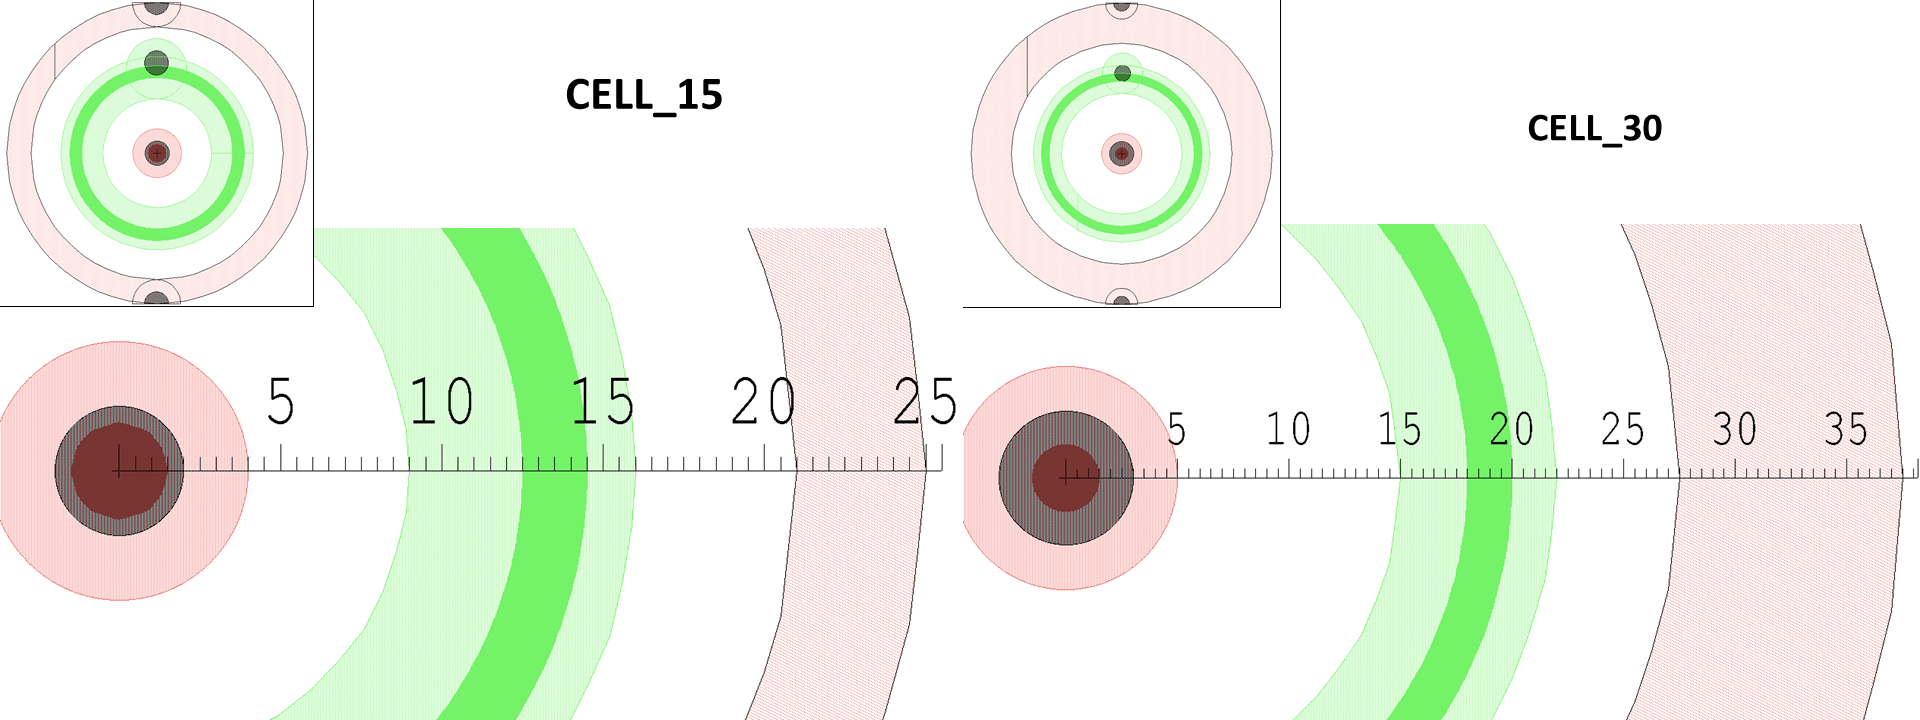
\includegraphics[width=1\textwidth]{3d-top-both.png}
	\caption{3DMiMic cell sizes. Distance scale is in $\mu$m.}
	\label{fig-top-both} 
\end{figure}

\begin{figure}
	\centering
	\begin{minipage}{.5\textwidth}
		\centering
		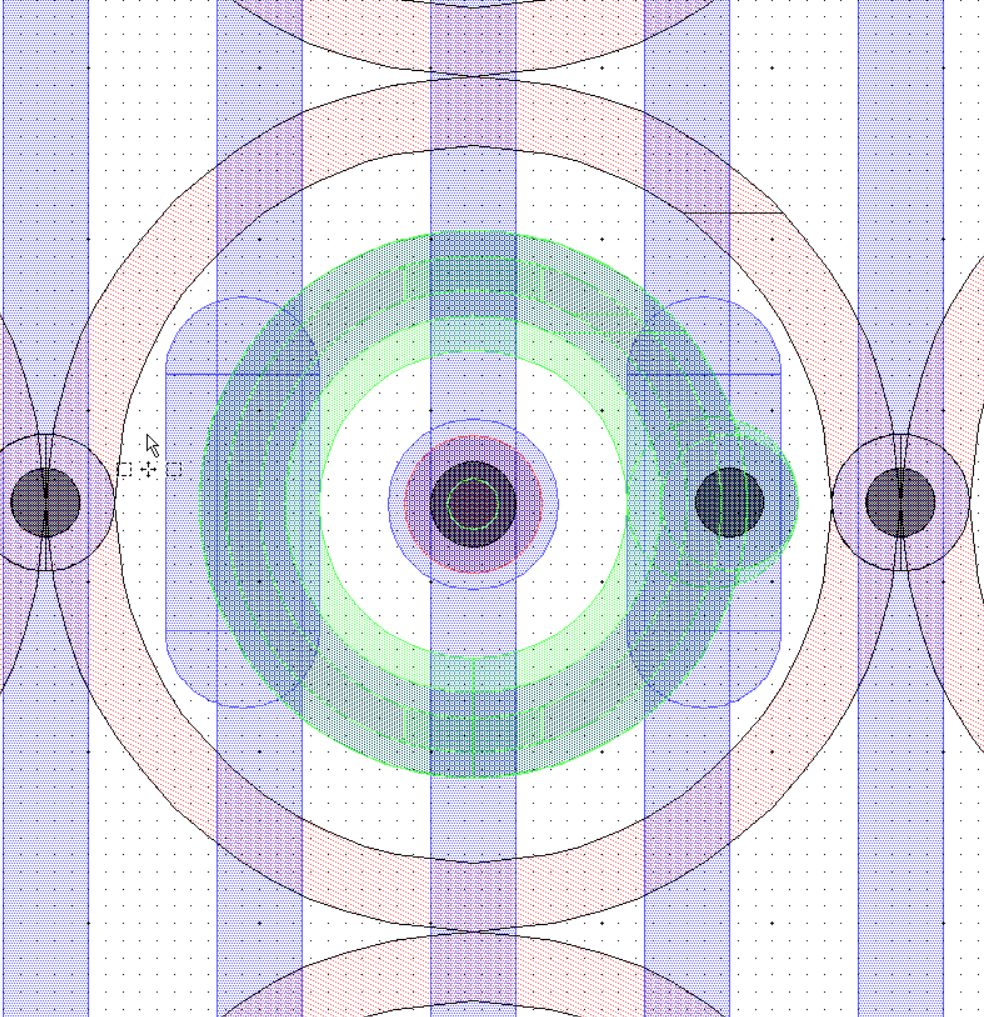
\includegraphics[width=.8\linewidth]{layout/MIC_ARRAY_1.png}
		\captionof{figure}{MIC$\_$ARRAY$\_$1 layout.}
		\label{fig-mic-array-1}
	\end{minipage}%
	\begin{minipage}{.5\textwidth}
		\centering
		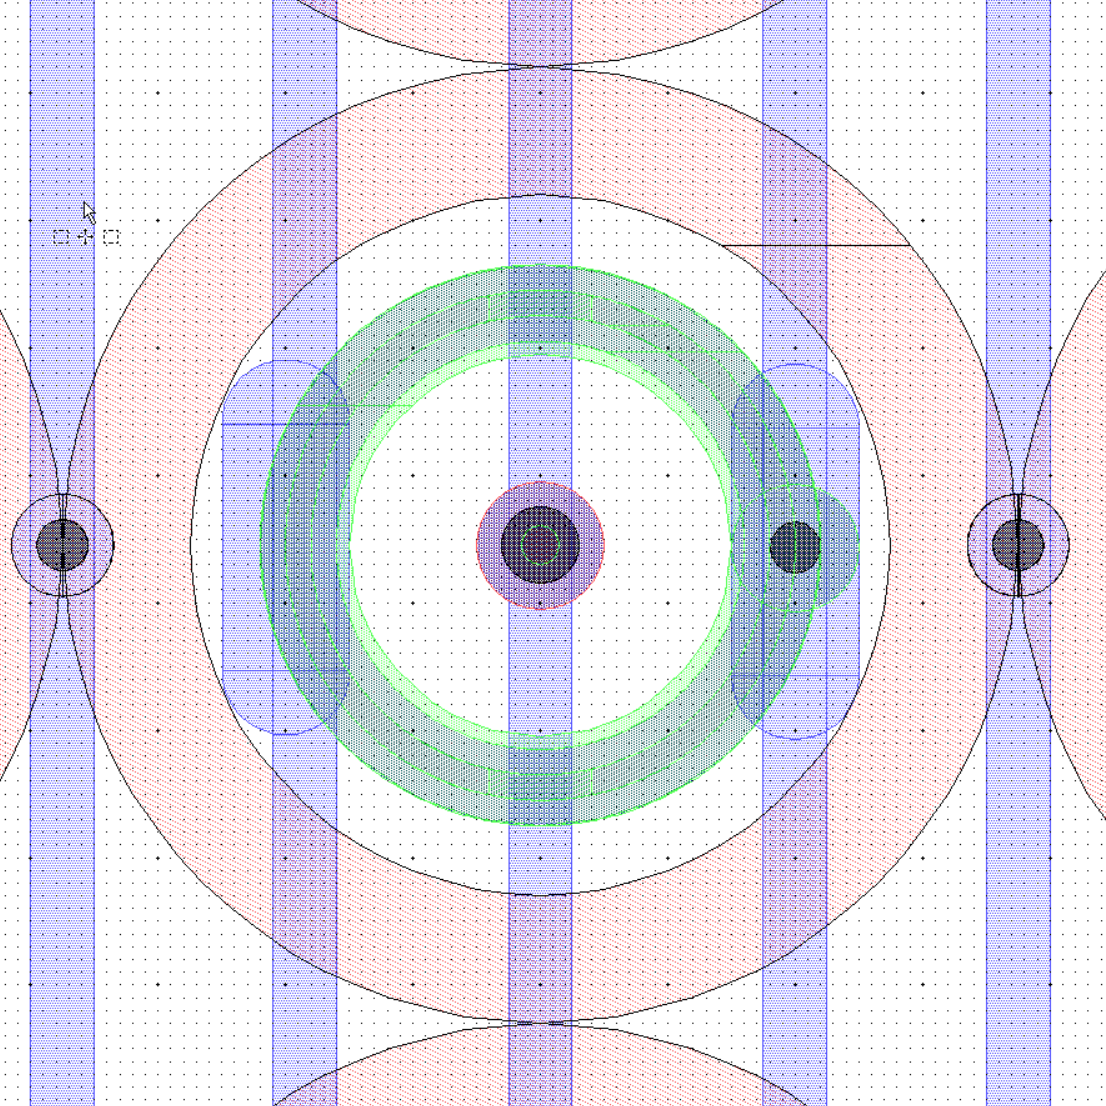
\includegraphics[width=.8\linewidth]{layout/MIC_ARRAY_1_L.png}
		\captionof{figure}{MIC$\_$ARRAY$\_$1$\_$L layout.}
		\label{fig-mic-array-1-L}
	\end{minipage}
\end{figure}

\begin{figure}
	\centering
	\begin{minipage}{.5\textwidth}
		\centering
		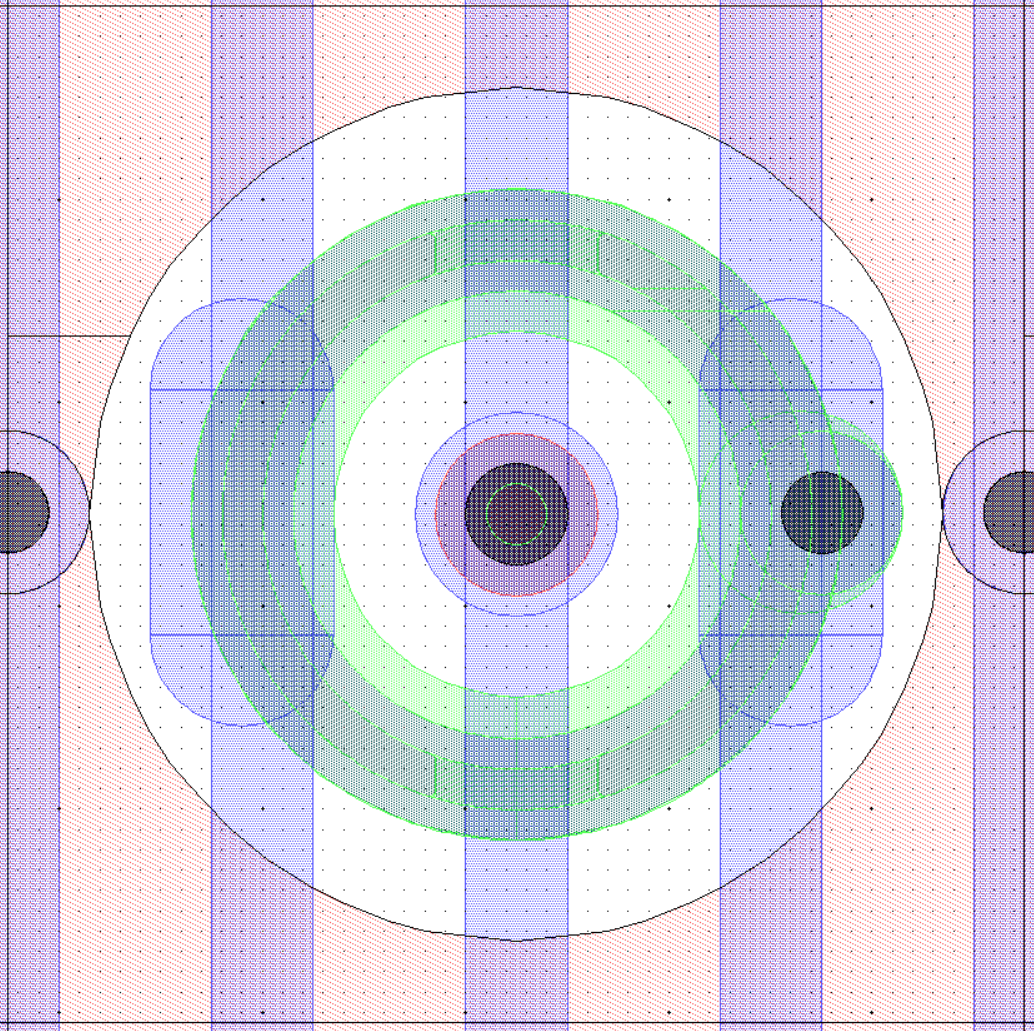
\includegraphics[width=.8\linewidth]{layout/MIC_ARRAY_2.png}
		\captionof{figure}{MIC$\_$ARRAY$\_$2 layout.}
		\label{fig-mic-array-2}
	\end{minipage}%
	\begin{minipage}{.5\textwidth}
		\centering
		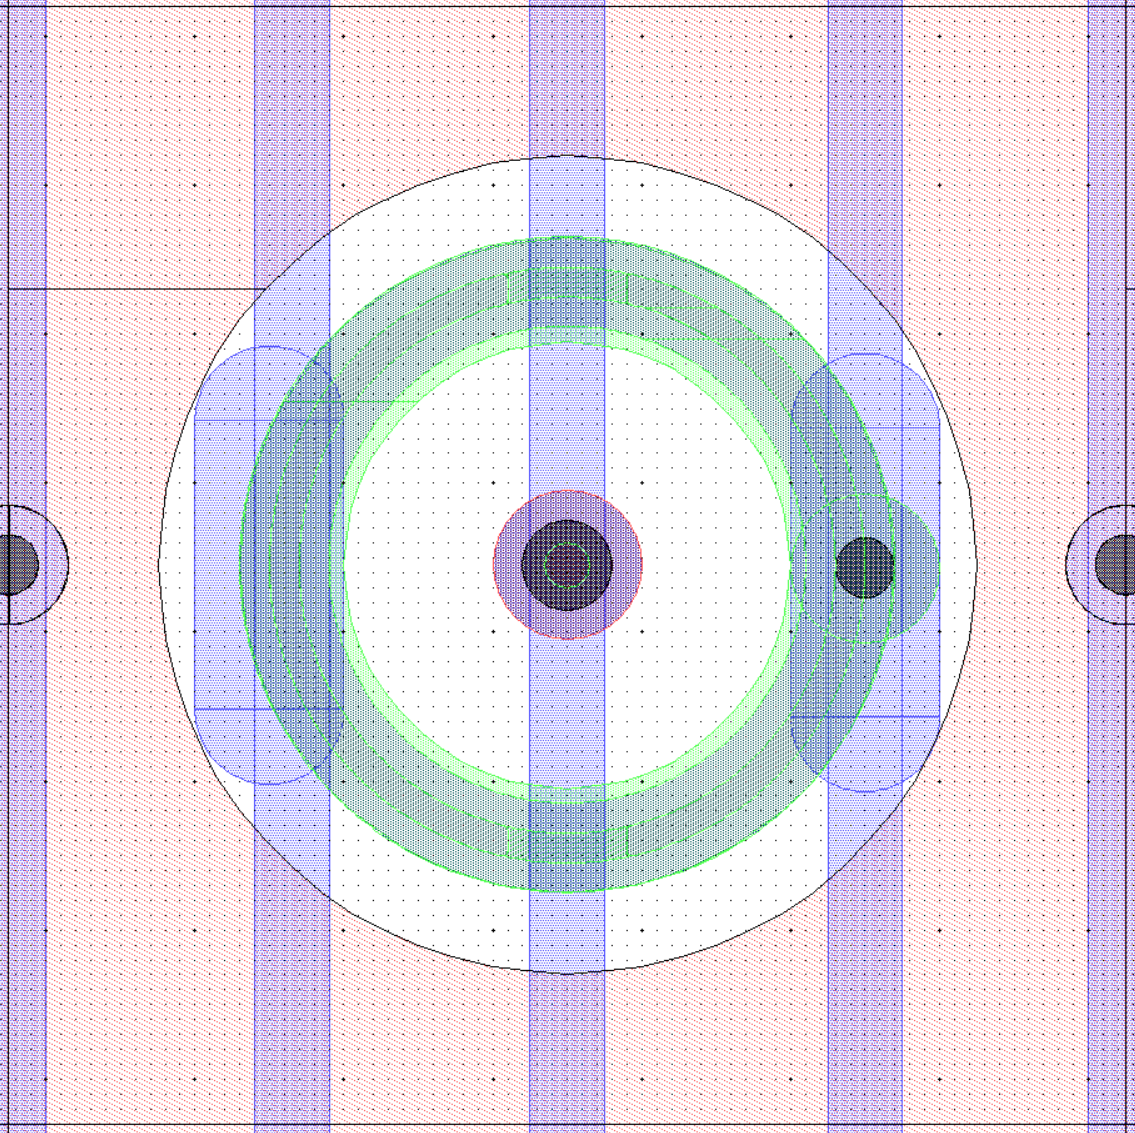
\includegraphics[width=.8\linewidth]{layout/MIC_ARRAY_2_L.png}
		\captionof{figure}{MIC$\_$ARRAY$\_$2$\_$L layout.}
		\label{fig-mic-array-2-L}
	\end{minipage}
\end{figure}

\begin{figure}
	\centering
	\begin{minipage}{.5\textwidth}
		\centering
		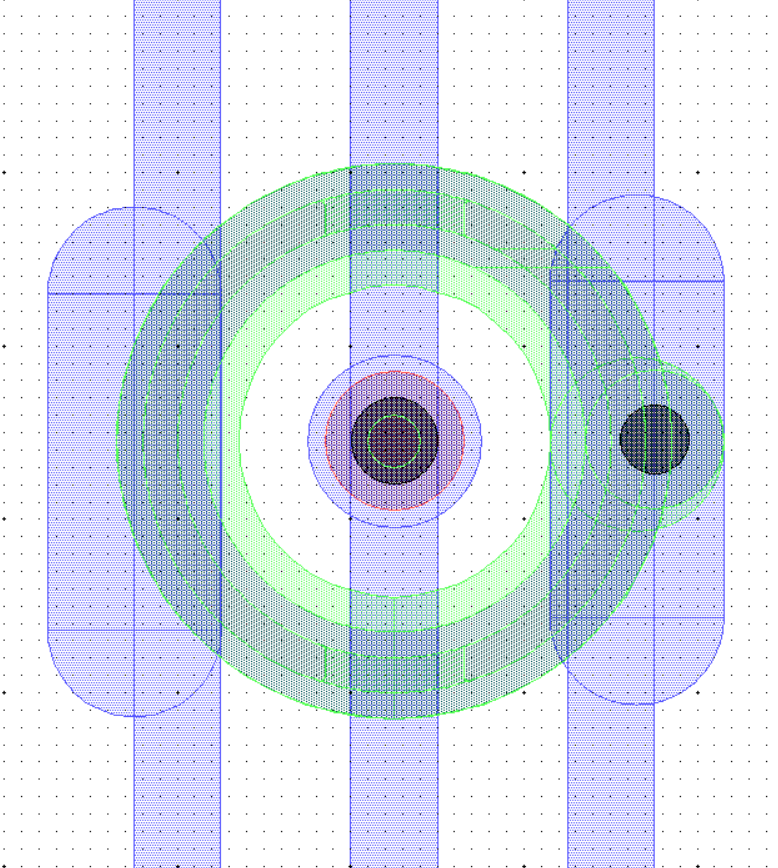
\includegraphics[width=.8\linewidth]{layout/MIC_ARRAY_3.png}
		\captionof{figure}{MIC$\_$ARRAY$\_$3 layout.}
		\label{fig-mic-array-3}
	\end{minipage}%
	\begin{minipage}{.5\textwidth}
		\centering
		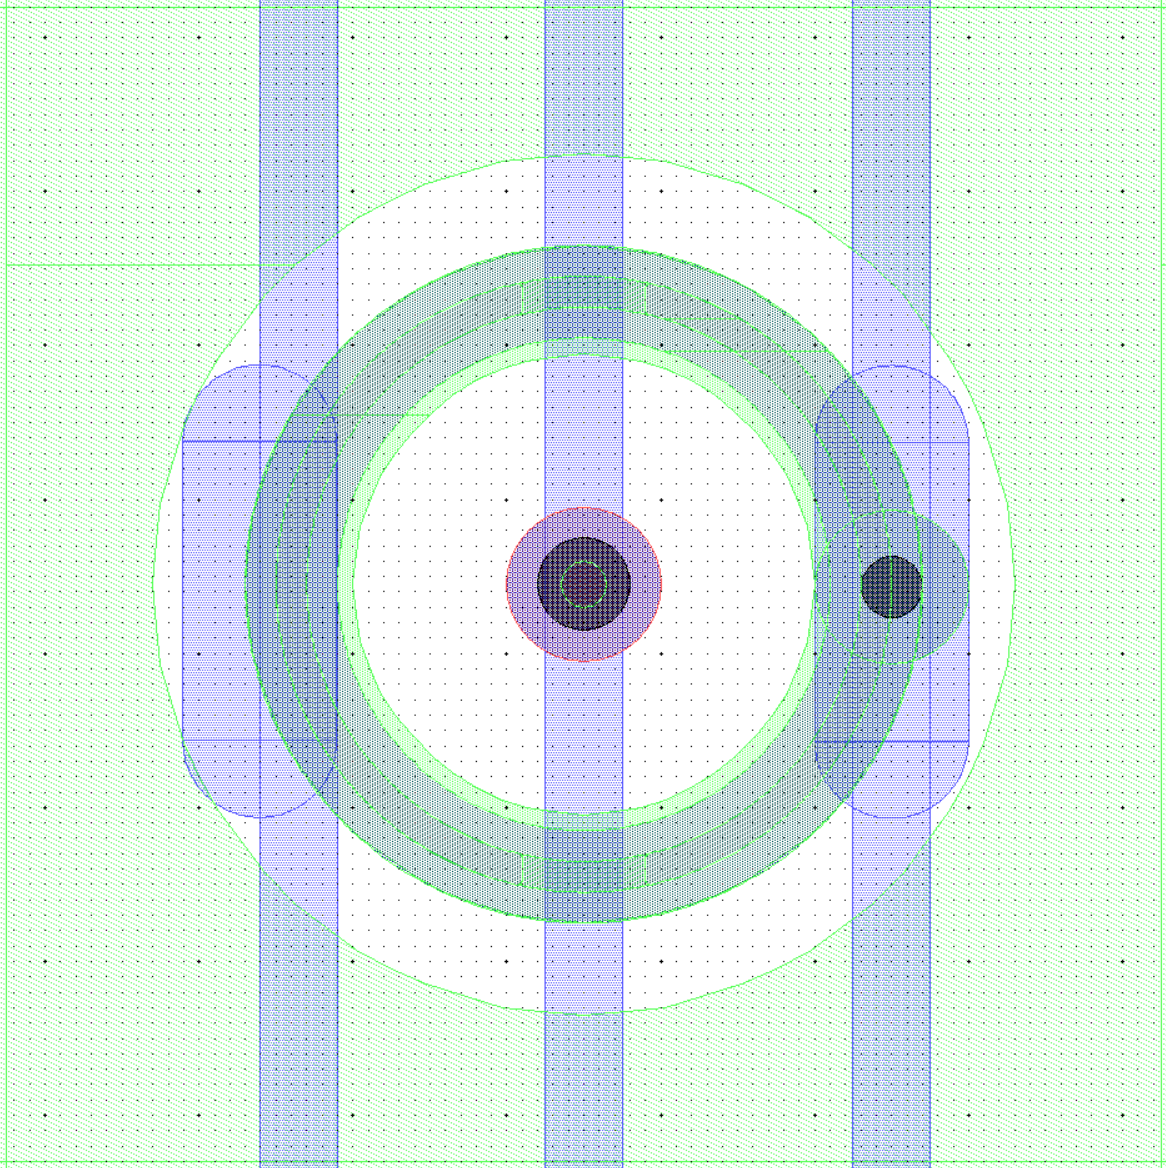
\includegraphics[width=.8\linewidth]{layout/MIC_ARRAY_3_L.png}
		\captionof{figure}{MIC$\_$ARRAY$\_$3$\_$L layout.}
		\label{fig-mic-array-3-L}
	\end{minipage}
\end{figure}

\begin{figure}
	\centering
	\begin{minipage}{.5\textwidth}
		\centering
		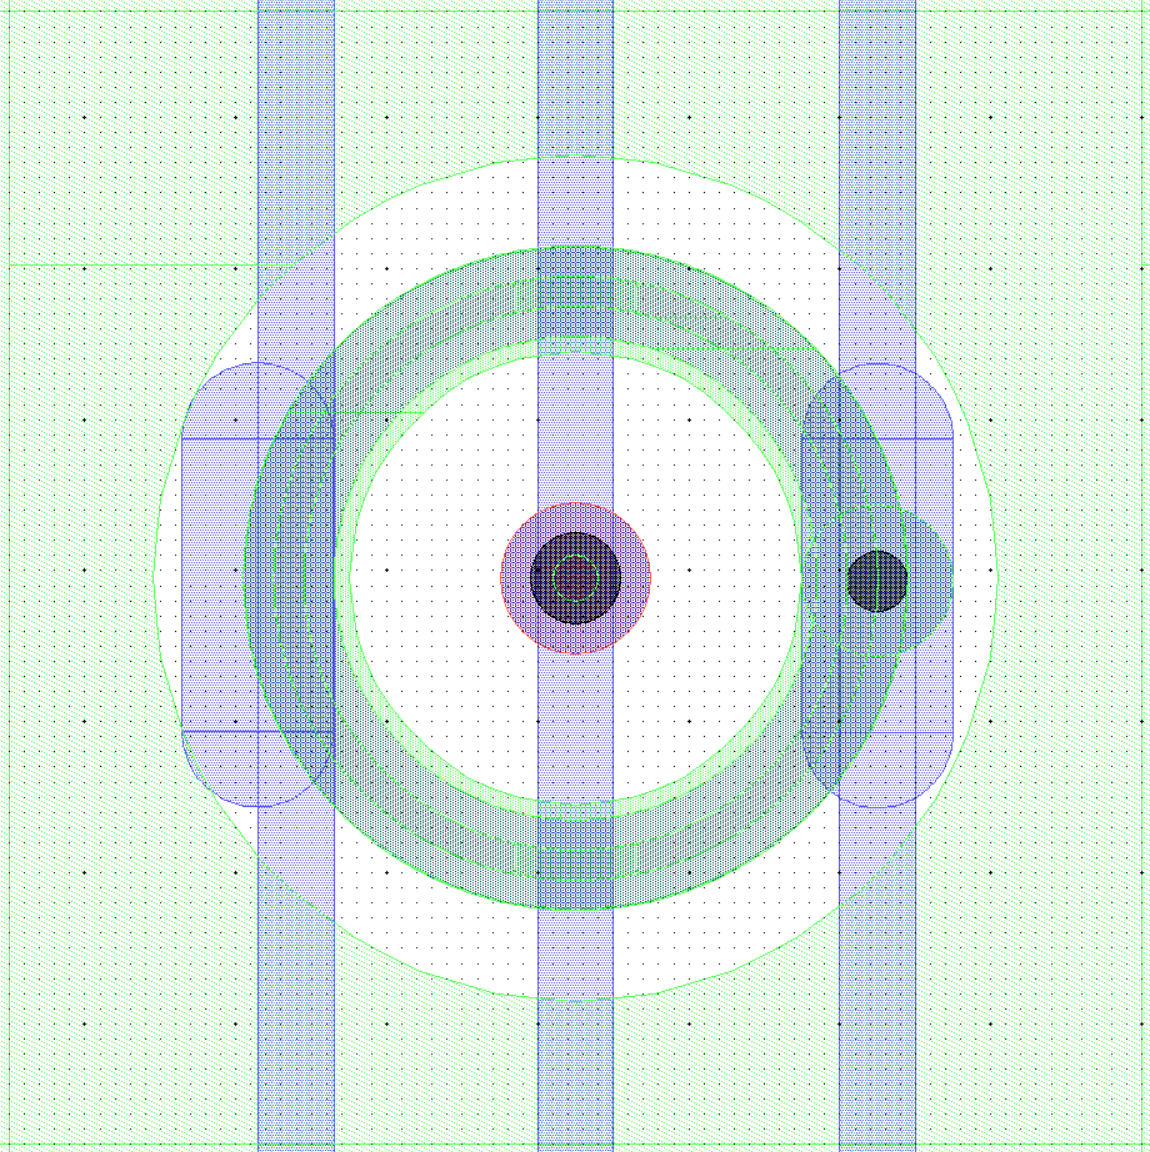
\includegraphics[width=.8\linewidth]{layout/MIC_ARRAY_3_PSTOP_L.png}
		\captionof{figure}{MIC$\_$ARRAY$\_$3$\_$PSTOP$\_$L layout.}
		\label{fig-mic-array-3-pstop-L}
	\end{minipage}%
	\begin{minipage}{.5\textwidth}
		\centering
		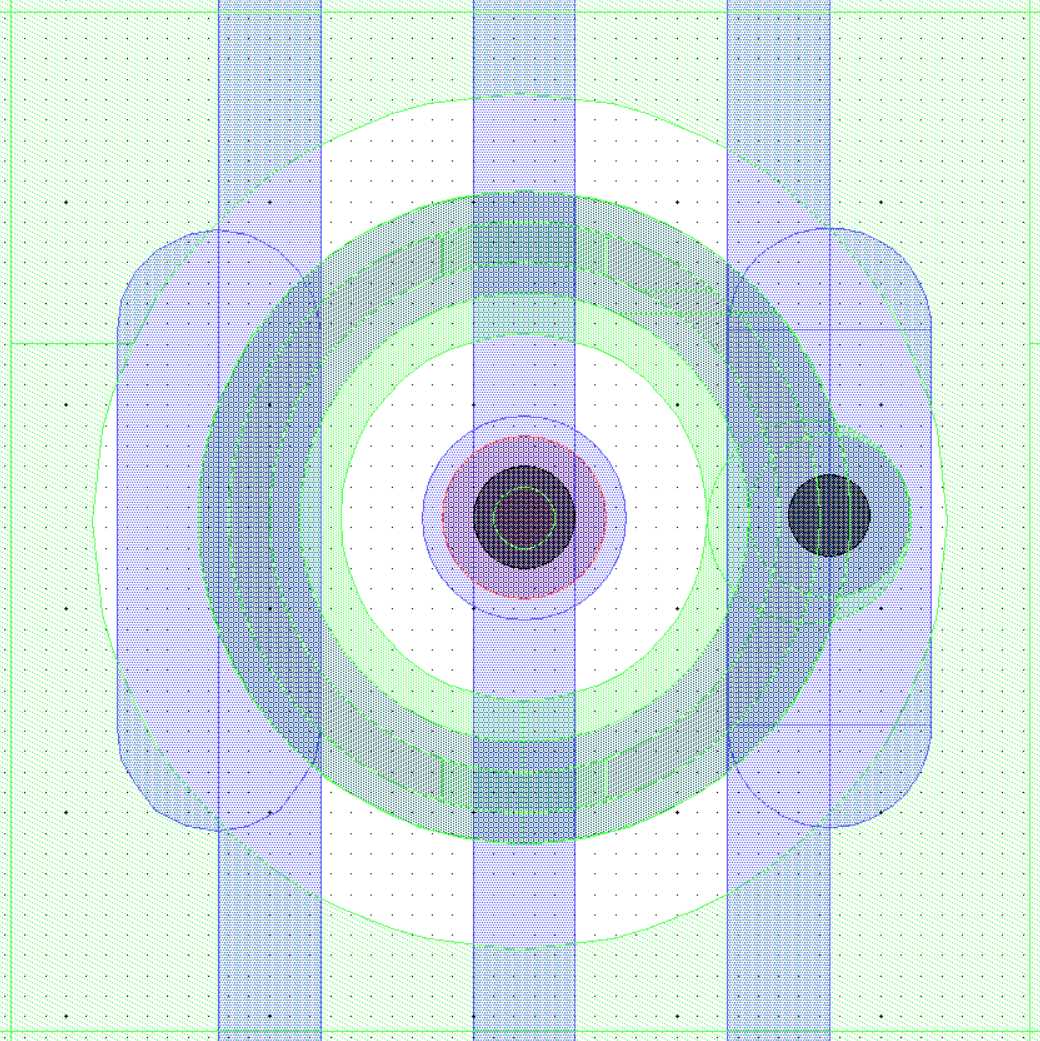
\includegraphics[width=.8\linewidth]{layout/MIC_ARRAY_PSTOP.png}
		\captionof{figure}{MIC$\_$ARRAY$\_$PSTOP layout.}
		\label{fig-mic-array-pstop}
	\end{minipage}
\end{figure}

\begin{figure}%[h]
	\centering
	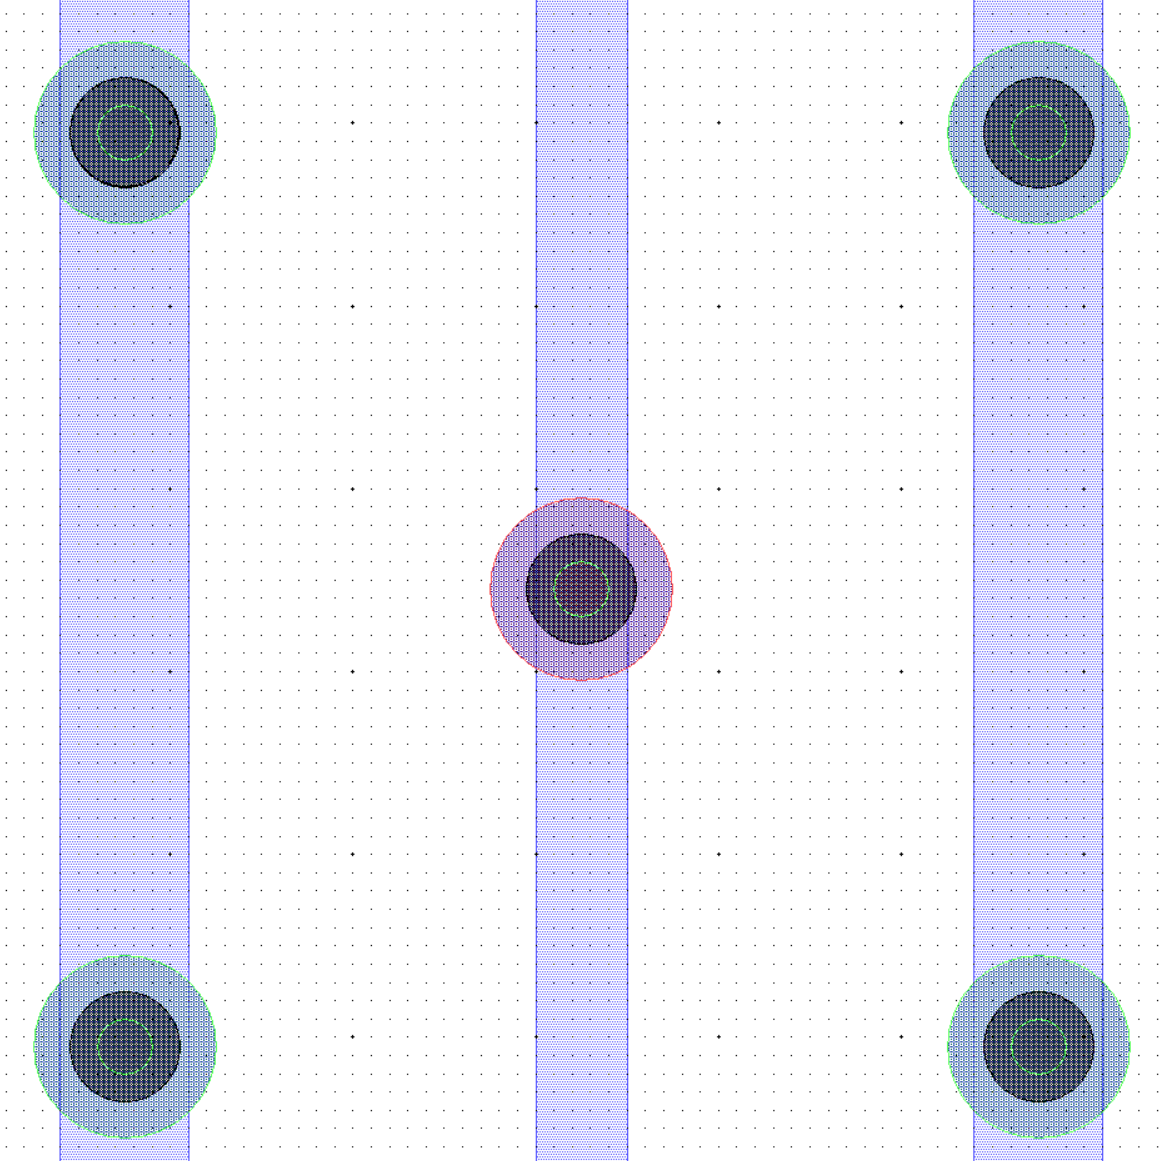
\includegraphics[width=0.35\textwidth]{layout/MIC_3D.png}
	\caption{MIC$\_$3D layout. Every second column is n+ or p+ pillars.}
	\label{fig-mic-3D} 
\end{figure}

\end{document}